\chapter{狭义相对论}

\section*{A 组}
\vspace{0.3cm}
\textbf{8-1} 在惯性系 $S$ 中观察到两事件同时发生, 空间间距为 1 $m$. 惯性系 $S'$ 沿两事件联线的方向相对于 $S$ 系运动, 在 $S'$ 系中观察到两事件之间的距离为 3 $m$. 试求 $S'$ 系相对 $S$ 系的速度大小和在 $S'$ 系中测得的两事件之间的时间间隔.


\vfill

\textbf{8-2} 如图所示, 在相对地面沿水平方向以匀速度 $v$ 高速运动的车厢内, 有一个由劲度系数为 $k$ 的轻弹簧和质量为 $m$ 的小物块构成的水平弹簧振子. 小物块从平衡位置开始, 以 $u \parallel v$ 的初速度在车厢内形成无摩擦的往返运动. 设 $u \ll c$ , 车厢中仍可用牛顿力学将振子的运动处理成简谐振动. 试用洛伦兹时空变换, 在地面系中计算振子在车厢中第一个四分之一振动周期内的运动过程经历的时间 $\Delta t_{1}$ 和第一个二分之一周期内的运动过程中经历的时间 $\Delta t_{2}$ .


\begin{center}
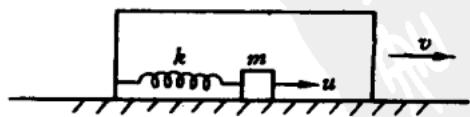
\includegraphics[width=0.3\textwidth]{figures/图8_1.jpg}
\end{center}

\vfill

\newpage

\textbf{8-3} 在以恒定速度 $v$ 沿平直轨道高速行驶的车厢中央有一旅客，已知他到车厢两端 $A$ 和 $B$ 的距离都是 $L_{0}$ . 今旅客点燃一根火柴，光脉冲向各个方向传播，并到达车厢两端 $A$ 和 $B$ . 设沿着车厢行驶方向， $A$ 端在前， $B$ 端在后，试在地面系用洛伦兹变换式计算光脉冲到达 $A, B$ 的时差 $\Delta t_{BA} = t_A - t_B$ 以及光脉冲到达 $A$ 端时车厢 $B$ 端和 $A$ 端之间的距离 $l_{BA}$ .


\vfill

\textbf{8-4} 地面中的水平隧道 $AB$ 长 $L_0$ , 一列火车 $A'B'$ 静长 $L > L_0$ . 今使火车如图所示, 以匀速度 $v$ 高速驶入隧道, 地面系中观察到 $A'$ 与 $A$ 相遇时恰好 $B'$ 与 $B$ 相遇. 试据洛伦兹变换式计算 $v$ 值, 并在列车系中计算从 $A, A'$ 相遇到 $B, B'$ 相遇之间经过的时间 $\Delta t'$ .


\begin{center}
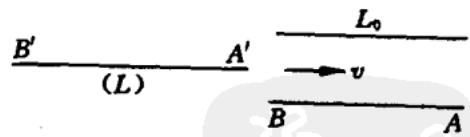
\includegraphics[width=0.3\textwidth]{figures/图_8_2.jpg}
\end{center}

\vfill

\newpage

\textbf{8-5} 静长同为 $L_{0}$ 的两把直尺 $AB, A'B'$ 沿长度方向相向而行，速度为 $v$ ，如图所示. 试据洛伦兹变换式在直尺 $AB$ 系中计算两尺相擦而过(从 $A'$ 与 $B$ 相遇到 $B'$ 与 $A$ 相遇)所经时间 $\Delta t$ .


\begin{center}
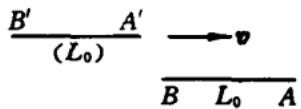
\includegraphics[width=0.2\textwidth]{figures/图8_3.jpg}
\end{center}

\vfill

\textbf{8-6} 一粒子在 $S'$ 系的 $x'y'$ 平面内以 $\frac{c}{2}$ 的恒定速度作直线运动，运动方向与 $x'$ 轴的夹角 $\theta' = 60^\circ$ 。已知 $S'$ 系相对 $S$ 系以速度 $v = 0.6c$ 沿 $x$ 轴运动，试据洛伦兹变换式求出粒子在 $S$ 系 $xy$ 平面上的运动轨迹，若为直线，再求出此直线的斜率。


\vfill

\newpage

\textbf{8-7} $S$ 系中有一静止时各边长为 $a$ 的正方形面板, 如图所示. 今使面板沿其对角线方向匀速运动, 速度大小为 $v$ . 某学生将 $\pmb{v}$ 沿面板静止时的两条直角边方向分解, 每一个方向上的分速度大小均为 $v' = v / \sqrt{2}$ . 考虑到每一直角边的长度收缩, 他认为 $S$ 系中运动面板的形状将如图所示, 是一个各边长为 $a' = \sqrt{1 - \beta'^2} a (\beta' = v'/c)$ 的正方形.

试分析地判定该学生的结论是否正确,并给出运动面板的正确形状及各边长度和面积.


\begin{center}
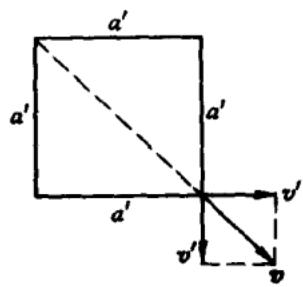
\includegraphics[width=0.2\textwidth]{figures/图_8_5.jpg}
\end{center}

\begin{center}
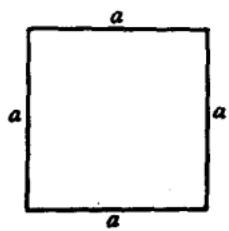
\includegraphics[width=0.2\textwidth]{figures/图8_4.jpg}
\end{center}

\vfill

\textbf{8-8} $\pi$ 介子静止时的平均寿命为 $2.5 \times 10^{-8} \mathrm{~s}$ , 在实验室中测得 $\pi$ 介子的平均运动距离为 $375 \mathrm{~m}$ , 试求 $\pi$ 介子相对实验室的速度.


\vfill

\newpage

\textbf{8-9} 静长为 $l$ 的飞船以恒定速度 $\pmb{v}$ 相对惯性系 $S$ 运动, 某时刻从飞船头部发出无线电信号, 试问飞船观察者认为信号经过多长时间到达飞船尾部? 再问 $S$ 系中的观察者认为信号经过多长时间到达飞船尾部?


\vfill

\textbf{8-10} 一艘宇宙飞船以 $0.8c$ 的速度于中午飞经地球, 此时飞船上和地球上的观察者都把自己的时钟拨到 12 点.

(1)按飞船上的时钟于午后12点30分飞船飞经一星际宇航站，该站相对地球固定，其时钟指示的是地球时间，试问按宇航站的时钟飞船何时到达该站？

(2) 试问按地球上的坐标测量,宇航站离地球多远?

(3) 于飞船时间午后 12 点 30 分从飞船向地球发送无线电信号,试问地球上的观察者何时(按地球时间)接收到信号?

(4)若地球上的观察者在接收到信号后立即发出应答信号，试问飞船何时(按飞船时间)接收到应答信号？


\vfill

\newpage

\textbf{8-11} 在某惯性系的一个平面上有两条相距 $H$ 的平行直线，另有一静长为 $L_{0} = \alpha H > H$ 的细杆. 今使细杆在该平面上作匀速运动, 速度 $\pmb{v}$ 的方向与两直线平行, 细杆与平行直线夹角为 $\phi$ , 而细杆恰好能在这两条平行直线之间运动, 即细杆两个端点分别靠近两条平行直线, 如图所示.

(1) 若 $\alpha$ 为定值, 试求 $\phi$ 与 $v$ 之间的函数关系;

(2) 确定 $\phi$ 的极小值 $\phi_{\min}$ 和极大值 $\phi_{\max}$ .


\begin{center}
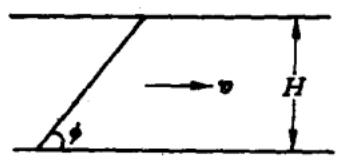
\includegraphics[width=0.2\textwidth]{figures/图_8_7.jpg}
\end{center}

\vfill

\textbf{8-12} 氢原子静止时发出的一条光谱线 $H_{\delta}$ 的波长为 $\lambda_{0}=410.1nm$ . 在极隧直射线管中，氢原子速率可达 $v=5\times10^{5}m/s$ ，试求此时在射线管前方的实验室观察者测得的谱线 $H_{\delta}$ 的波长 $\lambda$ .


\vfill

\newpage

\textbf{8-13} 静止的钾原子光谱中有一对容易辨认的吸收线($K$ 线和 $H$ 线), 其谱线的波长在 395.0 nm 附近. 来自牧夫星座一个星云的光中, 在波长为 447.0 nm 处发现了这两条谱线, 试求该星云远离地球的“退行速度”.


\vfill

\textbf{8-14} 如图所示, 实验室中粒子 $A$ 以 $\frac{4}{5}c$ 速度朝右运动, 粒子 $B$ 以 $\frac{4}{5} c$ 速度朝左运动. 试求随粒子 $A$ 运动的参考系测得的粒子 $B$ 运动速度大小.


\begin{center}
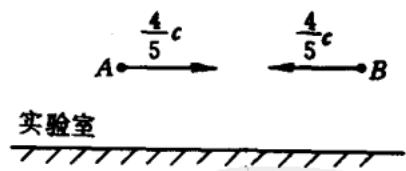
\includegraphics[width=0.2\textwidth]{figures/图8_9.jpg}
\end{center}

\vfill

\newpage

\textbf{8-15} 惯性系 $S'$ , $S$ 间的关系如常所设, 某光子在 $S'$ 系中沿 $y'$ 轴运动, 试由相对论速度变换式计算此光子在 $S$ 系中的速度分量 $u_{x}, u_{y}$ 以及速度大小 $u$, 以此验证相对论速度变换式符合光速不变原理.


\vfill

\textbf{8-16} 如图所示, $S$ 系中静止时的等腰直角三角板 ABC 沿其直角边 BC 方向匀速运动, 成为 $\angle C = 60^{\circ}$ 的直角三角板.

(1) 计算此三角板运动速度 $v$.

(2) 设某质点相对三角板以恒定的速率 $u$ 沿 AC 边运动:

(2. $A$) 若 AB 边长为 $l$，试求 $S$ 系测得的此质点从 $A$ 运动到 $B$ 的时间间隔 $\Delta t$ ;

(2.$B$) 再求 $S$ 系测得的此质点运动方向与 $BC$ 边延长线的夹角 $\phi$ , 证明 $\phi < 45^{\circ}$ ; 再以 $u \to 0, u = v, u \to c$ , 分别计算 $\phi$ 值.







\begin{center}
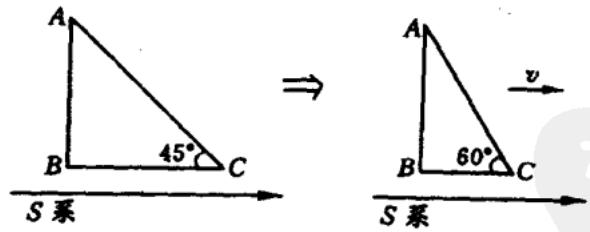
\includegraphics[width=0.2\textwidth]{figures/图8_10.jpg}
\end{center}

\vfill

\newpage

\textbf{8-17} 光在流动的水中传播, 在相对水静止的参考系中, 光的传播速度为 c/n, 已知水在实验室中的流速为 $v \ll c$ , 试求实验室中沿着水流方向和逆着水流方向分别测得的光速 $c_{+}$ 和 $c_{-}$ .


\vfill

\textbf{8-18} 如图所示, 一块玻璃板以速度 $v$ 向右运动. 在 $A$ 点有一闪光灯, 它发出的光通过玻璃板后到达 $B$ 点. 已知 $A$, $B$ 之间的距离为 $L$, 玻璃板在其静止的坐标系中的厚度为 $D$, 玻璃的折射率为 $n$, 试求光从 $A$ 点传播到 $B$ 点所需时间 $\Delta t$ . (只讨论光比玻璃板先到达 $B$ 点的情况.)

\begin{center}
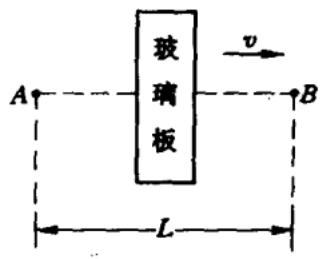
\includegraphics[width=0.2\textwidth]{figures/图_8_13.jpg}
\end{center}

\vfill

\newpage

\textbf{8-19} 惯性系 $S'$ 中在 $t_1' = t_2'$ 时刻，质点1和2分别位于 $x_1', y_1'$ 和 $x_2' = x_1', y_2' \neq y_1'$ 位置，速度分别为 $u_1' = 0$ 和 $u_2' = u_2'j$ ，受力分别为 $F_1' = F_{1y}'j$ 和 $F_2' = F_{2y}'j$ ，且有 $F_{2y}' = -F_{1y}'$ ，即有 $F_1' + F_2' = 0$ . 试证在惯性系 $S$ 中质点1和2也在同一时刻 $t_1 = t_2$ 受力 $F_1$ 和 $F_2$ ，但 $F_1 + F_2 \neq 0$ .

\vfill

\textbf{8-20} 一核弹含 $20\mathrm{kg}$ 的钚, 爆炸后生成物的静质量比原来小万分之一 $(1 / 10^{4})$ .

(1) 爆炸中释放了多少能量?

(2) 如果爆炸持续了 $1 \mu s$ ，平均功率多大？

\vfill

\newpage

\textbf{8-21} 聚变过程中 4 个氢核转变成 1 个氦核, 同时以各种辐射形式放出能量. 氢核质量 $1.0081 \mathrm{~u}$ (原子单位, $\mathrm{lu} = 1.66 \times 10^{-27} \mathrm{~kg}$ ), 氦核质量 $4.0039 \mathrm{~u}$ , 试计算 4 个氢核聚合为 1 个氦核时所释放的能量.

\vfill

\textbf{8-22} 某粒子在惯性系 $S$ 中具有的总能量为 500 MeV, 动量为 400 MeV/c, 而在惯性系 $S'$ 中具有的总能量为 583 MeV.

(1) 计算该粒子的静能；

(2) 计算该粒子在 $S'$ 系中的动量；

(3) 设 $S'$ 系相对 $S$ 系沿粒子运动方向运动, 试求 $S'$ 系相对 $S$ 系的运动速度.

\vfill

\newpage

\textbf{8-23} 静质量为 $m_{0}$ 的粒子在恒力作用下，从静止开始加速，经过 $\Delta t$ 时间，粒子的动能为其静能的 $n$ 倍。试求：

(1) 粒子达到的速度 $v$;

(2) 粒子获得的动量 $p$;

(3) 粒子所受冲量 $I$;

(4) 恒力大小 $F$.

\vfill

\textbf{8-24} 两个静质量相同的粒子,一个处于静止状态,另一个的总能量为其静能的4倍.当此两粒子发生碰撞后粘合在一起,成为一个复合粒子,试求复合粒子的静质量与碰撞前单个粒子静质量的比值.


\vfill

\newpage

\textbf{8-25} 如图所示, 一个以 0.8c 的速度沿 $x$ 方向运动的粒子衰变成两个静质量同为 $m_{0}$ 的粒子, 其中一个粒子以 0.6c 的速度沿 -y 方向运动. 若将衰变前粒子的静质量记为 $M_{0}$ , 试求:

(1) 另一个粒子运动速度的大小 $v$ 和方向角 $\theta$ ;

(2) 比值 $m_{0}/M_{0}$ .

\begin{center}
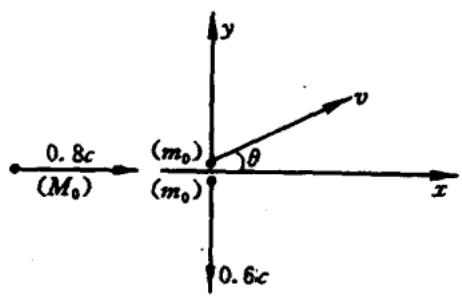
\includegraphics[width=0.3\textwidth]{figures/图8_14.jpg}
\end{center}

\vfill

\textbf{8-26} 氢原子基态能量为 $E_{0} = -13.6 \, eV$ ，氢原子 $n$ = 2, 3, … 激发态的能量为 $E_{n} = E_{0} / n^{2}$ 。实验室中两个处于基态的氢原子 1, 2 各以速度 $\boldsymbol{v}_{1}, \boldsymbol{v}_{2} (v_{1}, v_{2} \ll c)$ 朝着对方运动，碰撞后，沿原 $v_{1}$ 和 $v_{2}$ 方向分别发射出频率为 $\nu_{1}$ 和 $\nu_{2}$ 的光子，其中 $\nu_{1}$ 对应从 $n$ = 4 激发态跃迁到基态发射的光子频率， $\nu_{2}$ 对应从 $n$ = 2 激发态跃迁到基态发射的光子频率。发射后，两个氢原子静止地处于基态，试求 $v_{1}$ 和 $v_{2}$ 。

\vfill

\newpage

\textbf{8-27} 设有一处于激发态的原子以速度 $v$ 运动, 当其发射一个能量为 $E'$ 的光子后衰变至其基态, 并使原子处于静止状态, 此时原子的静质量为 $m_0$ . 已知激发态比基态能量高 $E_0$ , 试证:
\[
E ^ {\prime} = \left(1 + \frac {E _ {0}}{2 m _ {0} c ^ {2}}\right) E _ {0}.
\]
(原子激发态、基态能量均在原子静止时定义.)


\vfill

\textbf{8-28} 静质量为 $m_0$ 的质点, 开始时静止在 $x = A$ 处, 而后在线性回复力 $F_x = -kx$ ( $k$ 为正的常量) 作用下在 $x$ 轴上往返运动. 考虑相对论效应, 试求质点速率 $v$ 与所到位置 $x$ 的关系.


\vfill

\newpage

\textbf{8-29} 据爱因斯坦的广义相对论, 当星体中的物质因引力而塌缩到极小的球半径范围内时, 其周围的引力场可以强到使光子不能离开星体而去, 外部世界将“看”不到此星体, 称之为黑洞, 已知太阳、地球、电子质量分别为 $1.99 \times 10^{30} \mathrm{~kg}, 5.98 \times 10^{24} \mathrm{~kg}, 9.11 \times 10^{-31} \mathrm{~kg}$ , 假想通过挤压, 它们分别成为黑洞, 试估算各自的黑洞半径.


\vfill

\textbf{8-30} 三个惯性系 $S, S', S''$ 如图所示，其中 $S'$ 系沿 $S$ 系的 $x$ 轴以匀速度 $v$ 相对 $S$ 系运动， $x'$ 轴与 $x$ 轴重合， $y'$ 轴与 $y$ 轴平行。 $S''$ 系沿 $S'$ 系的 $y'$ 轴以匀速度 $v$ 相对 $S'$ 系运动， $y''$ 轴与 $y'$ 轴重合，$x''$ 轴与 $x'$ 轴平行. 三个坐标系的原点 $O, O', O''$ 重合时, 设定 $t = t' = t'' = 0$ . 试问 $S$ 系中任意 $t$ 时刻 $x''$ 轴在 $xy$ 平面上的投影是否为直线? 若为直线, 进而确定它的斜率.


\begin{center}
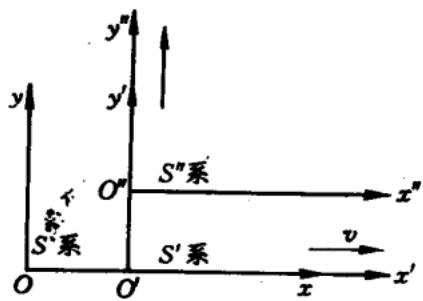
\includegraphics[width=0.3\textwidth]{figures/图8_15.jpg}
\end{center}

\vfill

\newpage

\textbf{8-31} 惯性系 $S, S''$ 间的相对关系如图所示， $O, O'$ 重合时 $t = t' = 0$ .

(1) 设在 $S'$ 系的 $O'x'y'$ 平面上有一个以 $O'$ 为中心、$R$ 为半径的固定圆环，试在 $S$ 系中写出 $t$ 时刻此圆环在 Oxy 平面投影曲线的方程；

(2) 在 $S'$ 系中从 $t' = 0$ 时刻开始有两个质点 $P_{1}$ 和 $P_{2}$ , 分别从 $x' = -R, y' = 0$ 和 $x' = R, y' = 0$ 位置以恒定的速率 $u$ 逆时针方向沿圆环运动, 试问:

(2. $A$) $S$ 系中 $P_{1}, P_{2}$ 各自在什么时刻 (分别记为 $t_{1}, t_{2}$ ) 开始运动?

(2.$B$) $S$ 系认为 $P_{1}, P_{2}$ 在什么时刻（记为 $t_{3}$ ）第一次相距最远？

(3) 导出 $S$ 系中质点 $P_{2}$ 沿 $x$ 轴的分运动 $x_{2}$ 与时间 $t$ 的函数关系，并在 $t \gg R / v$ 范围分析这一分运动的主要特征。（解答本小问时，建议引入参量 $\omega' = u / R$ .）


\begin{center}
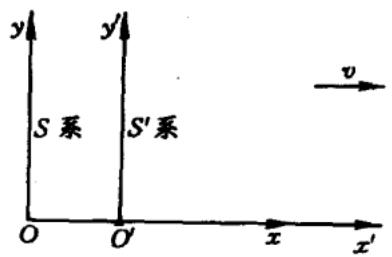
\includegraphics[width=0.3\textwidth]{figures/图8_16.jpg}
\end{center}

\vfill

\textbf{8-32} 惯性系 $S$, S' 间的相对运动关系如图所示, 两根细长的直尺 $AB$ 和 $A'B'$ 的静止长度相同，它们分别按图示方式静置于 $S$ 和 $S'$ 系中. 静止在 $A$ 和 $B$ 上的两个钟的计时率已按相对论的要求调好，静止在 $A'$ 和 $B'$ 上的两个钟的计时率也已按相对论的要求调好,但这四个钟的零点都是按下述方式确定的:当 $A$ 钟与 $A'$ 钟相遇时,两钟均调到零点;当 $B$ 钟与 $B'$ 钟相遇时,两钟均调到零点.

设 $A$ 与 $A'$ 相遇时, $A'$ 发出光信号, 已知 $B'$ 接收到光信号时, $B'$ 钟的读数为 1 个时间单位.

(1) 试问 $B$ 接收到光信号时, $B$ 钟的读数为多少时间单位?

(2) 若 $B'$ 接收到信号后, 立即发出应答光信号, 试问.

(2. $A$) $A'$ 接收到该应答信号时, $A'$ 钟的读数为多少时间单位?

(2.$B$) $A$ 接收到该应答信号时, $A$ 钟的读数为多少时间单位?

\begin{center}
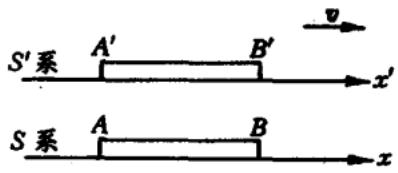
\includegraphics[width=0.3\textwidth]{figures/图_8_17.jpg}
\end{center}

\vfill

\newpage

\textbf{8-33} 飞船以 $v=\frac{3}{5}c$ 匀速度背离地球远行. 某时刻飞船朝着地球发出无线电信号, 经地球反射后又被飞船所接收, 飞船中观察者测得前后所经时间为 60 $s$.

(1) 飞船发信号时, 飞船系认为地球与飞船相距多远(记为 $l_{1}^{\prime}$ ), 地球系认为飞船与地球相距多远( $l_{1}$ )?

(2) 地球反射此信号时, 飞船系认为地球与飞船相距多远(记为 $l_{2}^{\prime}$ ), 地球系认为飞船与地球相距多远 ( $l_{2}$ )?

(3) 飞船接收到反射信号时, 飞船系认为地球与飞船相距多远 (记为 $l_{3}^{\prime}$ ), 地球系认为飞船与地球相距多远 ( $l_{3}$ )?

\vfill

\textbf{8-34} 宇航员乘宇宙飞船以 0.8c 的速度飞向 8 光年远、相对地球静止的星球，然后立即以同样速率返回地球。飞船上的钟在从地球出发时与地球上的钟同指零点，飞船运动换向时间忽略不计，设换向前后两瞬间飞船时钟读数相同。假定飞船于 2000 年元旦起飞，此后每年元旦宇航员和地球上的家人互发贺年电讯，家人自 2001 年元旦起共发 20 封贺电，试求两人各自收到对方贺电时自己钟表指示的时间。


\vfill

\newpage

\textbf{8-35} 如图所示, 光源 $S$ 向全反射体 $S'$ 发射一束平行光,发光功率为 $P_{0}$ . 设 $S'$ 以匀速度 $v$ 沿其法线方向朝 $S$ 运动, 试求 $S$ 接收到的反射光功率 $P$.


\begin{center}
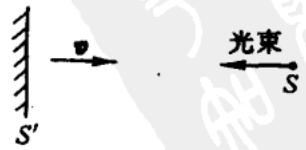
\includegraphics[width=0.3\textwidth]{figures/图8_20.jpg}
\end{center}

\vfill

\textbf{8-36} 如图所示, 在某太空惯性系 $S$ 中, 飞船 $A$ 和飞船 $B$以相同速率 $\beta c$ 作匀速直线航行, 飞船 $A$ 的航行方向与 $x$ 轴方向一致, 飞船 $B$ 的航行方向与 $x$ 轴负方向一致, 两飞船航线之间的距离为 $d$. 当 $A$ 和 $B$ 靠得最近时, 从 $A$ 向 $B$ 发出一束无线电联络信号.

(1) 为使 $B$ 能接收到信号, $A$ 中的宇航员认为发射信号的方向应与自己相对 $S$ 系的运动方向之间成什么样的夹角?

(2) 飞船 $B$ 中的宇航员接收到信号时, 认为自己与飞船 $A$ 相距多远?


\begin{center}
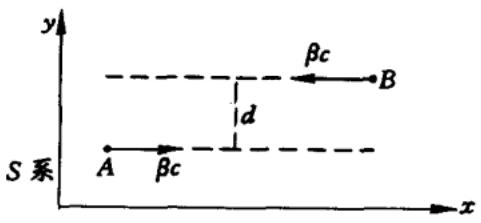
\includegraphics[width=0.3\textwidth]{figures/图_8_22.jpg}
\end{center}

\vfill

\newpage

\textbf{8-37} $S$ 系中有一个静止时各边长为 $l$ 的正方形ABCD面板，今使其沿 $AB$ 边方向匀速运动，速度为 $\pmb{v}$ ，如图所示.设质点 $P$ 从 $A$ 点出发，在面板参考系中以恒定的速率 $\pmb{u}$ 沿ABCD绕行一周.

(1) 分别在面板参考系和 $S$ 系中计算质点 $P$ 从 $A$ 点到 $B$ 点所经时间 $t_{AB}^{\prime}$ 和 $t_{AB}$ ;

(2) 分别在面板参考系和 $S$ 系中计算质点 $P$ 从 $B$ 点到 $C$ 点所经时间 $t_{BC}^{\prime}$ 和 $t_{BC}$ ;

(3) 分别在面板参考系和 $S$ 系中计算质点 $P$ 从 $A$ 点出发绕行一周所经时间 $t_{ABCD A}^{\prime}$ 和 $t_{ABCD A}$ .

\begin{center}
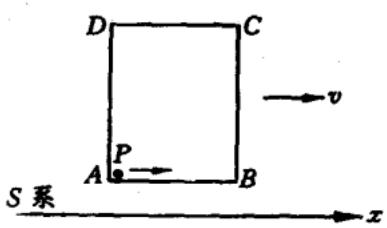
\includegraphics[width=0.3\textwidth]{figures/图_8_25.jpg}
\end{center}

\vfill

\textbf{8-38} 惯性系 $S$, $S'$ 间的相对关系如图所示，其中相对速度大小为 v=c/2，坐标原点 $O$, $O'$ 重合时， $t=t'=0$ .

(1) 设飞船 1 开始时静止于 $O'$ 点, 从 $t' = 0$ 时刻起, 在 $S'$ 系以恒定的加速度 $a_1$ 沿 $x'$ 轴运动, 试求飞船 1 在 $S$ 系中的运动方程 $x_1 - t$ .

(2) 设飞船 2 开始时静止于 $O$ 点, 从 t=0 时刻起, 沿 $x$ 轴正方向离开 $O$ 点，并在飞船 2 的瞬时静止惯性系（每一时刻相对飞船静止的惯性系）中，始终具有相同的加速度值 $a_{2}$ ，试求飞船 2 在 $S$ 系中的运动方程 $x_{2}-t$ .

(3) 设 $a_{2}=100a_{1}$ ，试问在 $S$ 系中飞船 2 何时追上飞船 1？

\begin{center}
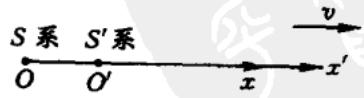
\includegraphics[width=0.3\textwidth]{figures/图_8_26.jpg}
\end{center}

\vfill

\newpage

\textbf{8-39} 宇宙飞船从地球出发沿直线飞向某恒星, 恒星距地球 $r = 3 \times 10^{4} \mathrm{l}. \mathrm{y}$ . 飞船的前一半航程中, 飞船在其瞬时静止惯性系中, 始终具有相同的加速度 $a' = 10 \mathrm{~m} / \mathrm{s}^{2}$ ; 飞船的后一半航程中, 飞船在其瞬时静止惯性系中以数值相同的加速度 $a'$ 作减速运动. 试问在飞船上测量, 整个航程经历了多长时间? 计算时只取一级近似.


\vfill

\textbf{8-40} 惯性系 $S, S'$ 之间的相对关系如图所示， $S$ 系与某星体连结在一起， $S, S'$ 系坐标原点 $O$ ， $O'$ 的间距远小于各自到其他星体的距离，在 $S, S'$ 系按常规方式分别引入以 $O, O'$ 为原点的球坐标角参量 $\{\theta, \phi\}$ ， $\{\theta', \phi'\}$ （图中未画出）。已知在 $S$ 系 $O$ 处的观察者看到的远处星体数呈各向同性分布，即单位立体角内观察到的星体数 $N$ 是一个与 $\{\theta, \phi\}$ 无关的常量，试求在 $S'$ 系 $O'$ 处的观察者在单位立体角内可观察到的星体数 $N'$ 的角分布，即函数关系 $N' - \theta', \phi'$ .

\begin{center}
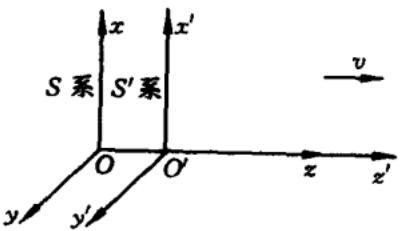
\includegraphics[width=0.3\textwidth]{figures/图8_27.jpg}
\end{center}

\vfill

\newpage

\textbf{8-41} 如图所示, 由介质 1 和介质 2 构成一界面, 两介质的折射率分别为 $n_1$ 和 $n_2$ , 界面的法线与 $S$ 系的 $x$ 轴平行. 现设界面随介质一起相对 $S$ 系以速度 $v$ 沿法线作匀速平动, 在 $S$ 系中入射光以入射角 $\theta_i$ 从介质 1 向界面入射, 反射角和折射角分别用 $\theta_{r}$ 和 $\theta_{t}$ 表示，试导出用入射光速 $u_{i}$ 和入射角 $\theta_{i}$ 表述的反射角 $\theta_{r}$ 和折射角 $\theta_{t}$ 的计算式.

\begin{center}
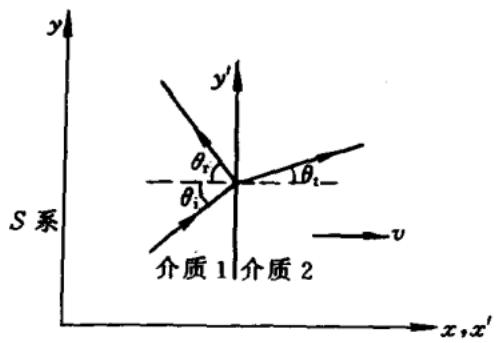
\includegraphics[width=0.3\textwidth]{figures/图_8_28.jpg}
\end{center}

\vfill

\textbf{8-42} 实验室中， $\alpha$ 粒子以 $v_{1} = \frac{4}{5} c$ 的速度射入厚度 $d = 0.35\mathrm{m}$ 的水泥防护墙，从墙射出时速度降为 $v_{2} = \frac{5}{13} c.$ 已知 $\alpha$ 粒子静质量 $m_0 = \frac{2}{3} \times 10^{-26}\mathrm{kg}$ ，墙对 $\alpha$ 粒子的作用力 $F_{0}$ 是常量，试求：

(1) $F_{0}$ ;

(2) 在以速度 $v_{1}$ 沿 $\alpha$ 粒子运动方向相对实验室运动的 $S'$ 系中测得的墙作用力 $F_{0}'$ ;

(3) 实验室和 $S'$ 系各自测得的 $\alpha$ 粒子通过墙的时间 $\Delta t$ 和 $\Delta t'$ .


\vfill

\newpage

\textbf{8-43} 据德布罗意波粒二象性假设, 动量为 $p$ 的自由运动实物粒子, 它所对应的实物粒子波的波长为 $\lambda = h/p$ , 其中 $h$ 为普朗克常量.

设有一个波长为 $\lambda_{\mathrm{i}}$ 的光子与一个运动的自由电子相碰，碰后电子静止，原光子消失，并产生一个波长为 $\lambda_0$ 的光子，运动方向与原光子运动方向成 $\theta = 60^{\circ}$ 的夹角。接着此光子又与另一个静止的自由电子相碰，碰后此光子消失，产生一个波长为 $\lambda_{\mathrm{f}} = 1.25 \times 10^{-10} \mathrm{~m}$ 的光子，运动方向与碰前光子运动方向成 $\theta = 60^{\circ}$ 角。试求第一个电子在碰前的德布罗意波长 $\lambda_{\mathrm{e}}$ 。

\vfill

\textbf{8-44} 太空火箭(包括燃料)的初始质量为 $M_{0}$ ，从静止起飞，向后喷出的气体相对火箭的速度 $u$ 为常量，任意时刻火箭相对地球速度为 $v$ 时火箭的瞬时静止质量记为 $m_{0}$ 。忽略地球引力影响，试求比值 $m_{0}/M_{0}$ 与速度 $v$ 之间的关系。

\vfill

\newpage

\textbf{8-45} 光子火箭是一种设想的航天器, 它利用“燃料”物质向后或向前辐射光束, 使火箭从静止加速或在运动中向前加速或减速.

设光子火箭从地球起飞时静止质量(包括燃料)为 $M_{0}$ ，朝着与地球相距 $R=1.8\times10^{6}$ $l$.$y$.的仙女座星云飞行。要求火箭在25年(火箭时间)后“软着陆”到达目的地。不计所有引力影响，略去火箭加速和减速所经时间，试求：

(1) 火箭相对地球匀速段的飞行速度 $v$;

(2) 火箭出发时的静止质量 $M_{0}$ 和到达目的地时的静止质量 $M_{0}^{\prime}$ 之间的比值.

\vfill

\textbf{8-46} 如图所示, 在一次粒子碰撞实验中, 观察到一个低速 $\mathbf{K}^{-}$ 介子与一个静止质子 $\mathfrak{p}$ 发生相互作用，生成一个 $\pi^{+}$ 介子和一个未知的$X$粒子，在匀强磁场 $B$ 中 $\pi^{+}$ 介子和$X$粒子的轨迹已在图中画出.已知 $B = 1.70\mathrm{T}$ 测得 $\pi^{+}$ 介子轨迹的曲率半径为 $R_{1} =$ $34.0\mathrm{cm}$

(1) 试确定 $X$ 粒子轨迹的曲率半径 $R_{2}$ ;

(2) 试参考下表确认 $X$ 为何种粒子.

\begin{center}
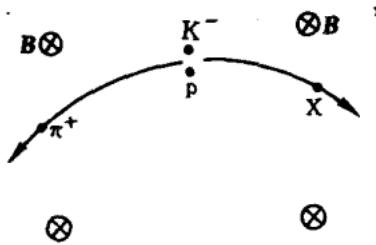
\includegraphics[width=0.2\textwidth]{figures/图8_31.jpg}
\end{center}

\begin{table}[htbp]
\centering
\begin{tabular}{|c|c|c|}
\hline
粒子符号 & 静能/MeV & 电荷/$e$ \\
\hline
$\mathrm{e}^+, \mathrm{e}^-$ & 0.511 & $1, -1$ \\
$\mu^+, \mu^-$ & 105.7 & $1, -1$ \\
$\pi^+, \pi^-$ & 139.6 & $1, -1$ \\
$\mathrm{K}^+, \mathrm{K}^-$ & 493.8 & $1, -1$ \\
$\mathrm{p}$ & 938.3 & $1$ \\
$\mathrm{n}$ & 939.6 & $0$ \\
$\Lambda^0$ & 1115.4 & $0$ \\
$\Sigma^+$ & 1189.4 & $1$ \\
$\Sigma^0$ & 1192.3 & $0$ \\
$\Sigma^-$ & 1197.2 & $-1$ \\
$\Xi^0$ & 1314.3 & $0$ \\
$\Xi^-$ & 1320.8 & $-1$ \\
$\Omega^-$ & 1675 & $-1$ \\
\hline
\end{tabular}
\end{table}

\vfill

\newpage

\textbf{8-47} $\mu^{-}$ 子的电量 $q = -e(e = 1.6 \times 10^{-19} \mathrm{C})$ ，静质量 $m_0 = 100 \mathrm{MeV} / c^2$ ，静止时的寿命 $\tau_0 = 10^{-6} \mathrm{s}$ . 设在地球赤道上空距地面高度 $h = 10^4 \mathrm{~m}$ 处有一个 $\mu^{-}$ 子以接近于真空光速的速度垂直向下运动.

(1) 试问此 $\mu^{-}$ 子至少应有多大的总能量才可到达地面?

(2) 若把赤道上空 $10^{4}$ $m$ 高度范围内的地球磁场处理成水平匀强磁场, $B=10^{-4}$ $T$, 试求上述已获得能量的 $\mu^{-}$ 子在到达地面时的偏离方向和总的偏转角.

\vfill

\textbf{8-48} 某粒子的静止质量为 $m_0$ ，以初速 $v_0$ 从 $t = 0$ 开始沿 $x$ 轴方向运动，运动期间始终受到一个指向 $y$ 轴方向的恒力 $\pmb{F}$ 的作用。试证，任意 $t > 0$ 时刻粒子的两个速度分量为
\[
v _ {x} = \frac {v _ {0}}{\sqrt {1 - v _ {0} ^ {2} / c ^ {2}}} \sqrt {c ^ {2} / (c ^ {2} + k)}, \quad v _ {y} = \frac {F t}{m _ {0}} \sqrt {\frac {c ^ {2}}{c ^ {2} + k}},
\]
\[
k = \frac {v _ {0} ^ {2}}{1 - v _ {0} ^ {2} / c ^ {2}} + \left(\frac {F t}{m _ {0}}\right) ^ {2},
\]
进而证明，当 $t \to \infty$ 时，速率 $v \to c, v_x \to 0$ .


\vfill

\newpage

\textbf{8-49} 在惯性系某个 $S$ 平面上的 $O$ 点有一个带电量为 $Q > 0$ 的固定点电荷，另一个带负电荷 $-q$ 的质点 $P$ 受点电荷 $Q$ 的库仑力作用，绕 $O$ 点在 $S$ 平面上作有界曲线运动. 设 $P$ 点的初始相对论能量为 $E_0, P$ 点相对 $O$ 点的初始角动量为 $L_0$ ，且有
\[
q Q / 4 \pi \varepsilon_ {0} L _ {0} c \ll 1,
\]
其中 $c$ 为真空光速.

(1) 试证在零级近似下, 即在 $qQ / 4\pi \varepsilon_0 L_0 c \approx 0$ 的条件下, $P$ 点的运动轨道是一个椭圆;

(2) 试证 $P$ 点的真实运动是带有进动的椭圆运动, 并求出 $P$ 点相对 $O$ 点的径矢长每变化一周对应的进动角 $\Delta\theta$ .

\newpage


\textbf{8-50} 引力红移和恒星质量的测定

(1) 频率为 $\nu$ 的一个光子具有惯性质量, 此质量由光子的能量确定. 在此假定下, 光子也有引力质量, 量值等于惯性质量. 与此相应, 从一颗星球表面向外发射出的光子, 逃离星球引力场时, 便会损失能量.
试证明，初始频率为 $\nu$ 的光子从星球表面到达无穷远处，若将它的频移(频率增加量)记为 $\Delta \nu$ ，则当 $|\Delta \nu| \ll \nu$ 时，有
$$
\frac {\Delta \nu}{\nu} \approx - \frac {G M}{R c ^ {2}},
$$
式中 $M$ 为星球质量， $R$ 为星球半径。这样，在距星球足够远处对某条已知谱线频率红移的测量，可用来测出比值 $M / R$ ，如果知道了 $R$ ，星球的质量 $M$ 便可确定。

(2) 在一项太空实验中发射出一艘无人驾驶的宇宙飞船, 欲测量银河系中某颗恒星的质量 $M$ 和半径 $R$ . 飞船径向地接近目标时, 可以监测到从星球表面 $\mathbf{H}_{\mathrm{e}}^{+}$ 离子发射出的光子对飞船实验舱内的 $\mathbf{H}_{\mathrm{e}}^{+}$ 离子束进行共振激发. 光子被共振吸收的条件是飞船 $\mathbf{H}_{\mathrm{e}}^{+}$ 离子朝着星球的速度必须与光子的引力红移严格地相适应. 共振吸收时的飞船 $\mathbf{H}_{\mathrm{e}}^{+}$ 离子相对星球的速度 $v$ (记为 $v = \beta c$ ), 可随着飞船到星球表面最近距离 $d$ 的变化而进行测量, 实验数据在下面表格中给出. 请充分利用这些数据, 试用作图法求出星球的半径 $R$ 和质量 $M$ . 解答中不必进行误差计算.

\begin{table}[htbp]
\centering
\caption{数据表}
\label{tab:data_grid}
\begin{tabular}{|l|c|c|c|c|c|}
\hline
速度参量 $\beta/10^{-5}$ & 3.352 & 3.279 & 3.195 & 3.077 & 2.955 \\ \hline
到星球表面距离 $d/10^{8}$m & 38.90 & 19.98 & 13.32 & 8.99 & 6.67 \\ \hline
\end{tabular}
\end{table}

(3) 为在本实验中确定 R 和 M，通常需要考虑因发射光子时离子的反冲造成的频率修正（热运动对发射谱线仅起加宽作用，不会使峰的分布移位）：

(3. A) 令 $\Delta E$ 为原子(或者说离子)在静止时的两个能级差, 假定静止原子在能级跃迁后产生一个光子并形成一个反冲原子. 考虑相对论效应, 试用能级差 $\Delta E$ 和初始原子静止质量 $m_0$ 来表述发射光子的能量 $h\nu$ .

(3.B) 现在, 试对 $\mathbf{H}_{\mathrm{e}}^{+}$ 离子这种相对论频移比值 $(\Delta \nu / \nu)_{\text{反冲}}$ 作出数值计算. 计算结果应当得出这样的结论, 即反冲频移远小于(2)问中得到出的引力红移.
计算用常量：
$H_{e}^{+}$ 的静能量： $m_{0}c^{2}=4\times938\,MeV$ ;
$H_{e}^{+}$ 的能级： $E_{n}=-(4\times13.6/n^{2})\mathrm{eV}, n=1,2,3,\cdots.$ 
(第 26 届 IPhO(国际中学生物理奥林匹克)试题)
356 
